\section{Robuster PI-Regler mit SISO-Tool}
\begin{figure}[h!]
    \centering
    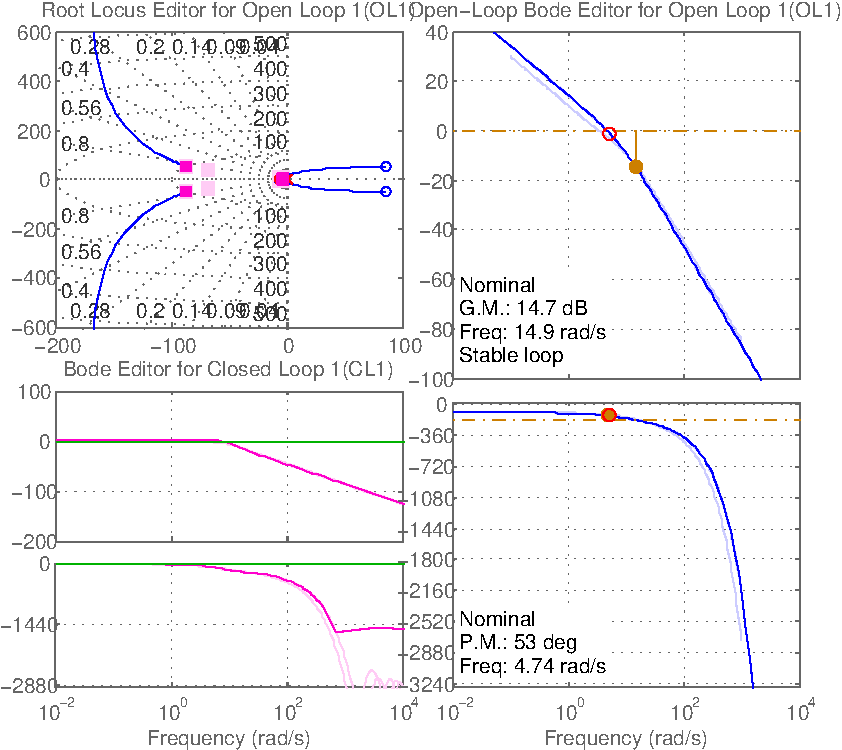
\includegraphics[width=0.8\textwidth]{10/diag_siso_pi.pdf}
    \caption{Bode- und Nyquistdiagramm}
    \label{fig:07a}
\end{figure}
\begin{figure}[h!]
    \centering
    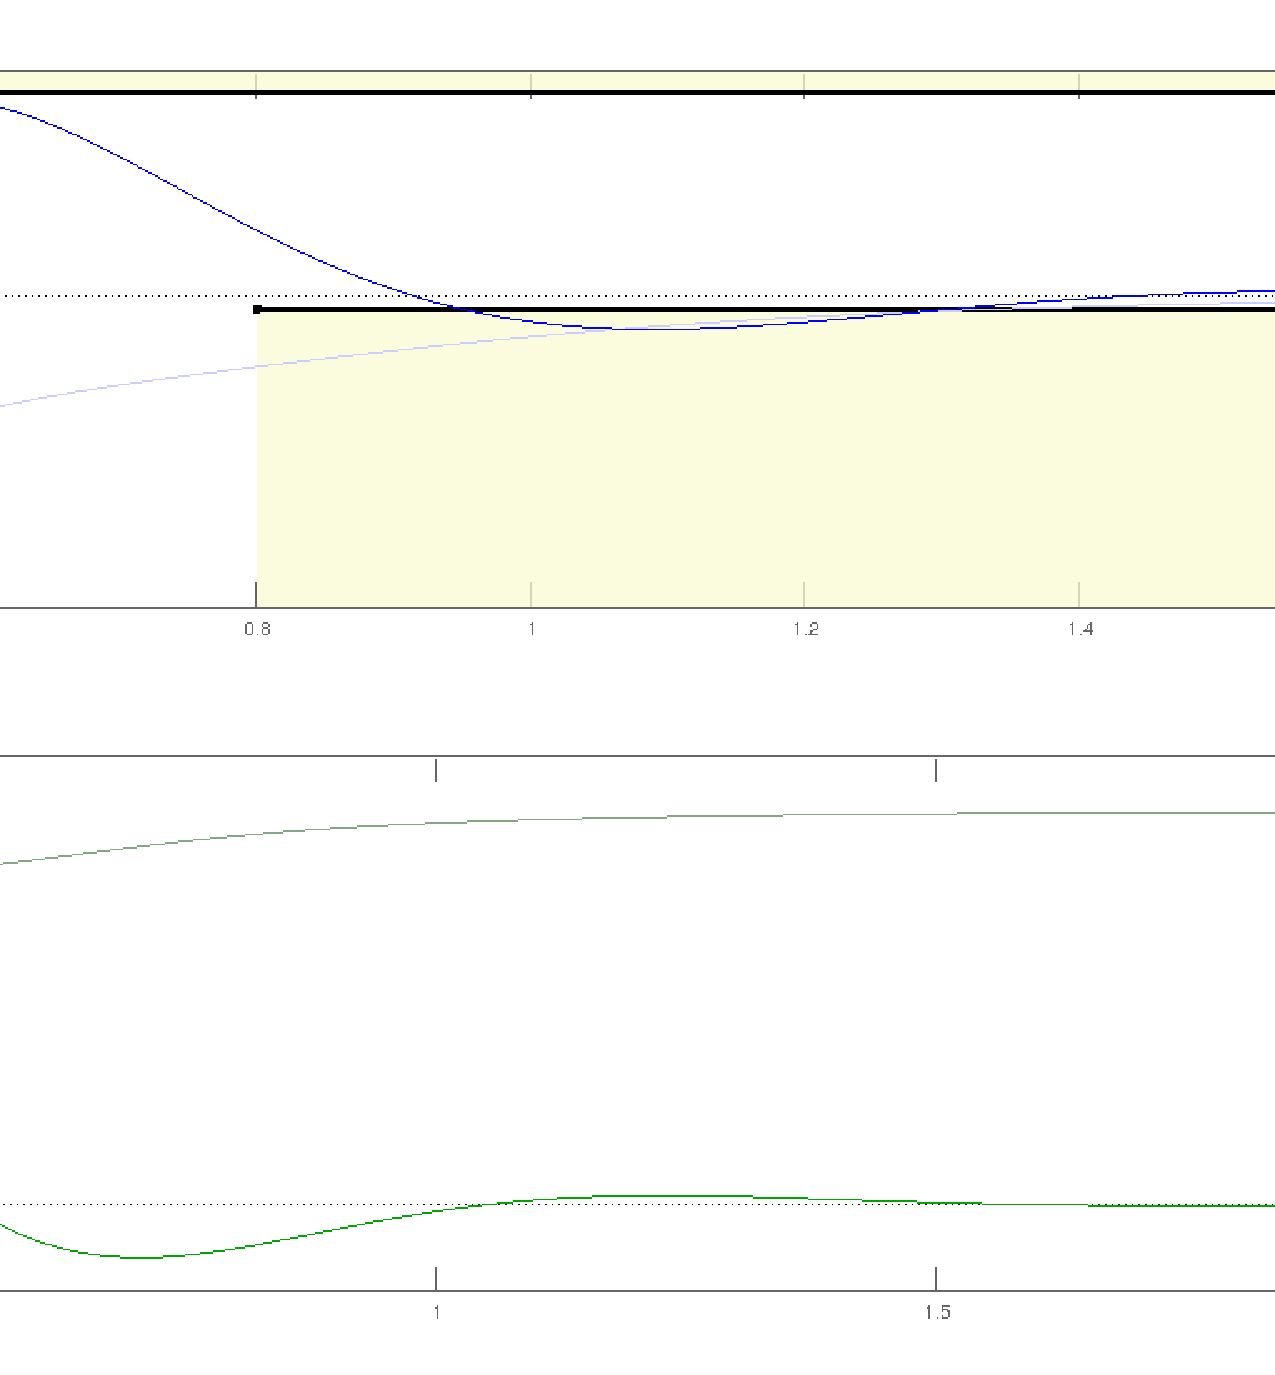
\includegraphics[width=0.7\textwidth]{10/step_siso_pi.pdf}
    \caption{Schrittantwort}
    \label{fig:07b}
\end{figure}
\begin{figure}[h!]
    \centering
    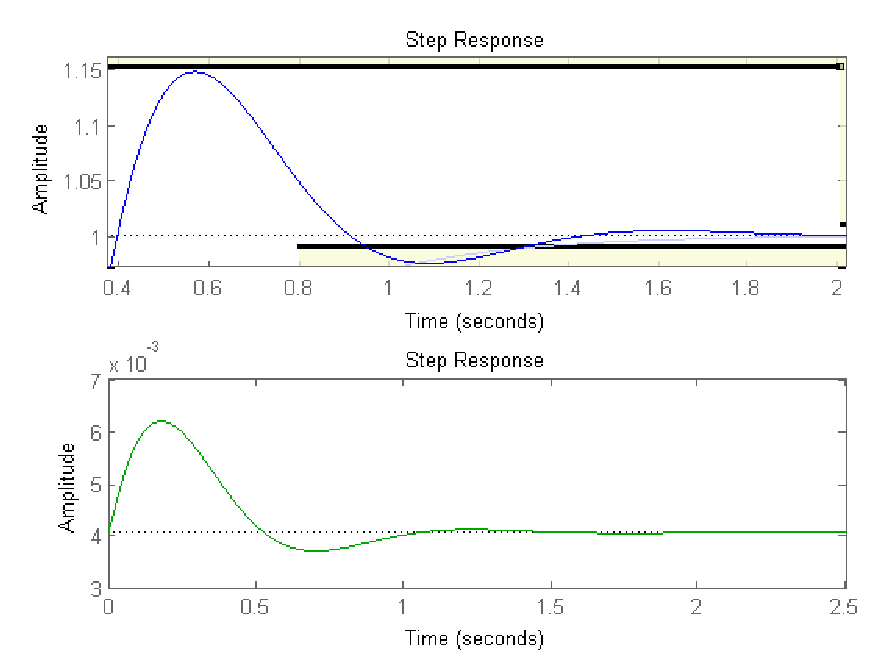
\includegraphics[width=0.7\textwidth]{10/step_detail_siso_pi.pdf}
    \caption{Detail Schrittantwort}
    \label{fig:07c}
\end{figure}
\begin{table}[h!]
    \centering
    \begin{tabular}{l|ll}
        Stabilitätsreserve  & $G_1$                     & $G_2$ \\
        \hline
        Amplitudenreserve   & $14.7~[\si{\deci\bel}]$   & $15.7~[\si{\deci\bel}]$ \\
        Phasenreserve       & $53~[\si{\degree}]$       & $76.1~[\si{\degree}]$ \\
    \end{tabular}
\end{table}
